\documentclass[a4paper, 12pt]{article}
\usepackage[linesnumbered,ruled,vlined]{algorithm2e}
\usepackage[margin=2.53cm]{geometry}  % Marges normales de Word
\usepackage[french]{babel}  % Langue
\usepackage[utf8]{inputenc}  % Saisi du texte : permet les accents
\usepackage[T1]{fontenc} 	% Encodage du document
\setlength{\parindent}{0pt}  % Pas d'indentation
\setlength{\parskip}{1em}  % Passer une ligne après chaque paragraphe
\usepackage{hyperref}	% Inclure les liens
\usepackage{graphicx}	% Inclure des images
\topskip0pt  % Permet \vspace*{\fill} pour centrer verticalement
\usepackage{xcolor} % Texte coloré
\usepackage{ragged2e}       % Justification du texte
\usepackage{tocloft}
\usepackage{enumitem}
\usepackage{float}
\usepackage{geometry}
\usepackage{fancyhdr}
\usepackage{amsmath}
\usepackage{listings}
\usepackage{tikz}
\usepackage{longtable}
\usepackage{algorithm}
\usepackage{algpseudocode}

\renewcommand{\sfdefault}{phv}  % Arial pour le texte sans-serif

\fancyhead[L]{Système de Recommandation de Livres} % Left-aligned header text
\fancyhead[R]{} % Right header (empty)
\renewcommand{\headrulewidth}{0.3pt} % Line under the header
\renewcommand{\footrulewidth}{0.3pt} % No line in the footer

% Définir l'espacement entre le titre et le numéro de page
\renewcommand{\cftsecnumwidth}{2.5em} % Largeur du numéro de section
\renewcommand{\cftsubsecnumwidth}{3.0em} % Largeur du numéro de sous-section
\renewcommand{\cftsubsubsecnumwidth}{3.5em} % Largeur du numéro de sous-sous-section
\hyphenpenalty=10000

\begin{document}

\makebox[\textwidth][c]{
    \begin{minipage}[t]{20cm} % Set the minipage width to 20cm
\hspace{0.2cm}
        
\includegraphics[width=20cm]{enTete-esi.png} % Image is exactly 20cm wide
    \end{minipage}
}

\vspace{1cm}
\begin{center}
\thispagestyle{empty}
    \textsc{\LARGE Ecole Supérieure en Informatique 08-MAI-1945 Sidi Bel Abbes}\\[1cm]
    
    \textsc{\Large Rapport de mini projet}\\[0.5cm]
    
    \rule{\linewidth}{0.5mm} \\[0.4cm]
    {\huge \bfseries Système de Recommandation de Livres}\\
    \rule{\linewidth}{0.5mm} \\[1.5cm]
    \vfill
\begin{minipage}{0.4\textwidth}
        \begin{flushleft} \large
            Présenté par :\\
            \begin{itemize}[label=\textbullet]
    \item  Ghandouz Amina
      \item  Benghenima Hafsa
      \item  Benahmed Firdaws
    
\end{itemize}
        \end{flushleft}
    \end{minipage}
    ~
\hspace{2.5cm}
    \begin{minipage}{0.4\textwidth}
        \begin{flushright} \large
             Encadrant :\\
            \textbf{ Dr. Nassima DIF}
        \end{flushright}
    \end{minipage}\\[2cm]
	\vfill
    
    {\large Date de publication : Décembre 2024}\\
\end{center}
\newpage
\setcounter{page}{1}
\newpage

% ********************************************** Somaire *****************************************************************************
\tableofcontents % Génère la table des matières
\newpage
%**********************************************Introduction ***********************************************************************
\pagestyle{fancy}
\begin{minipage}{\textwidth}

\section{Introduction}

\vspace{1cm}
\justifying

\hspace{1cm}Les systèmes de recommandation font partie intégrante de nos vies, ils nous aident à mieux acheter, trouver du nouveau contenu, etc. Pour les entreprises, ces systèmes sont un outil essentiel pour augmenter leurs ventes et la satisfaction des clients.

La majorité des bibliothèques n’ont pas de systèmes de recommandation de livres, ce qui les empêche de faire découvrir aux utilisateurs des livres qui pourraient les intéresser. Par conséquent, si les bibliothèques pouvaient recommander automatiquement des livres, elles pourraient mieux promouvoir la lecture.\vspace{0.5cm}

Le but de ce projet est de créer un système de recommandation de livres basé sur les livres que les utilisateurs lisent et qui ont des intérêts similaires.\vspace{0.5cm}

Les retombées du projet seraient d’avoir un système fonctionnel pouvant être intégré aux bibliothèques, permettant aux utilisateurs de découvrir des livres intéressants qu’ils ne connaissaient pas.\vspace{0.5cm}

Dans ce projet, nous explorons les techniques d’apprentissage automatique non supervisé, en particulier les algorithmes d’association, pour développer un système de recommandation de livres. Nous avons expérimenté trois algorithmes : \textbf{Apriori}, \textbf{ECLAT}, et \textbf{FP-Growth}, afin de découvrir les associations les plus pertinentes entre les livres. Après une analyse comparative, nous avons sélectionné le meilleur modèle et l'avons déployé pour fournir des recommandations efficaces.\vspace{0.5cm}

Le code complet du projet est disponible sur GitHub via le lien :\vspace{0.2cm}

\url{https://github.com/hafsabn/Book-Recommendation-System}
\end{minipage}

%********************************************************************************************************************************
\newpage
\pagestyle{fancy}
\begin{minipage}{\textwidth}

\section{Type de Système de Recommandation}

\vspace{0.5cm}
\justifying

\hspace{1cm}Le système de recommandation que nous avons développé utilise des algorithmes basés sur les règles d'association, en particulier Apriori, Eclat, et FP-Growth, qui sont des techniques de découverte d'ensembles fréquents.\vspace{0.5cm}

Dans ce type de système, nous identifions des ensembles de livres fréquemment lus ensemble par plusieurs utilisateurs. Lorsque qu'un utilisateur a lu un livre qui fait partie de ces ensembles fréquents, nous lui recommandons l'autre livre du même ensemble. Par exemple, si un ensemble fréquent est formé des livres A et B (lisent ensemble souvent par les utilisateurs), et qu'un utilisateur a déjà lu le livre A, le système recommande automatiquement le livre B.
\end{minipage}


%**********************************************************************************************************************************
%\begin{minipage}{\textwidth}
\vspace{1cm}


\section{Sources de Données Utilisées}

\justifying 

Nous avons utilisé deux datasets principaux pour ce projet : \texttt{books\_df} et \texttt{ratings\_df}. 
\begin{itemize}[label=\textbullet]
\item Le dataset \texttt{book\_df} contient 271 360 lignes et 8 colonnes, représentant les informations relatives aux livres, telles que le titre, l'auteur...
\item Le dataset \texttt{ratings\_df} contient 1 149 780 lignes et 3 colonnes, représentant les évaluations des utilisateurs. Chaque ligne associe un identifiant d'utilisateur User-ID, un identifiant de livre ISBN, et une évaluation (rating).
\end{itemize}

\vspace{0.5cm}
Nous avons filtré le dataset \texttt{ratings\_df} pour ne conserver que les évaluations dont la note est supérieure à 5. Cette étape permet de se concentrer uniquement sur les livres ayant reçu des évaluations relativement positives, afin d'éviter d'inclure des évaluations faibles qui pourraient biaiser les recommandations. Ensuite, nous avons fusionné ce sous-ensemble avec le dataset \texttt{books\_df} en utilisant l'ISBN comme clé de jointure. Cela nous a permis d’obtenir un dataset final contenant à la fois les titres des livres et leurs évaluations positives, essentiel pour générer des recommandations précises. 

\begin{figure}[H]
    \centering
    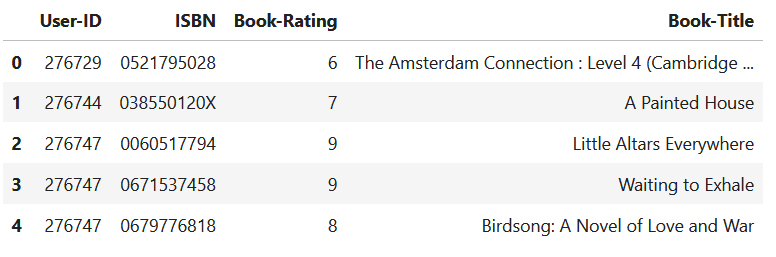
\includegraphics[width=0.9\textwidth]{final-df.png} % Remplace 'image.png' par le nom de ton image
    \caption{Extrait du dataset final fusionné.}
    \label{fig:mon_image}
\end{figure}

\vspace{1cm}

\newpage
\pagestyle{fancy}
\section{Prétraitement et Nettoyage des Données}

\justifying 
Après la fusion des datasets, nous avons effectué un nettoyage pour préparer les données avant de les utiliser pour les recommandations. Plusieurs étapes ont été réalisées pour garantir la qualité du dataset fusionné :
\begin{itemize}[label=\textbullet]
\item    Doublons : Des doublons ont été identifiés, notamment des évaluations répétées pour un même utilisateur et un même livre. Ces doublons ont été supprimés afin de garantir l'intégrité des données.

\item    Valeurs manquantes : Aucune valeur manquante n'a été trouvée dans les colonnes essentielles du dataset. Par conséquent, ce problème n'a pas nécessité de traitement particulier.

\item    Filtrage des évaluations : Nous avons sélectionné uniquement les évaluations supérieures à 5, afin de nous concentrer sur les livres ayant reçu des évaluations positives.
\end{itemize}
Ces étapes ont permis d'obtenir un dataset propre et prêt à être utilisé pour les recommandations.

\vspace{0.5cm}
Afin de visualiser les effets du nettoyage, nous avons comparé la distribution des évaluations avant et après le prétraitement:


\begin{figure}[H]
    \centering
    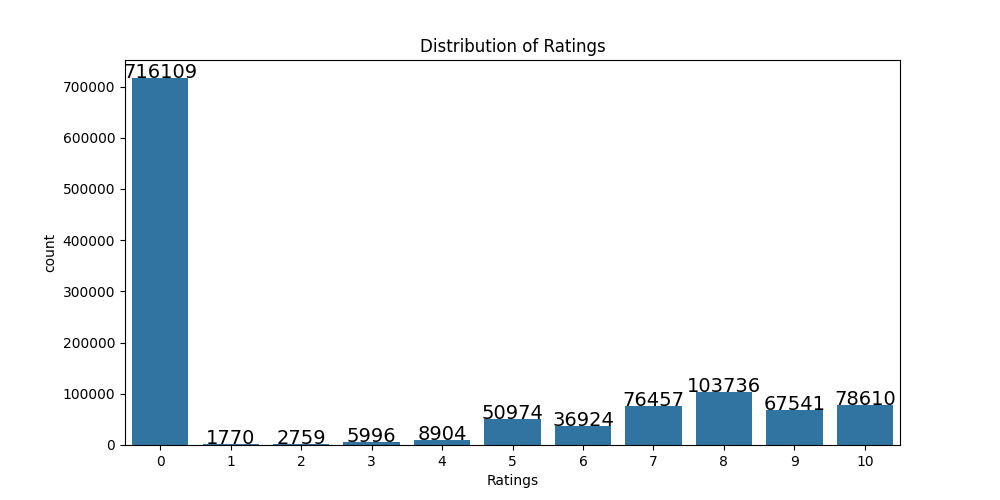
\includegraphics[width=0.9\textwidth]{distribution_of_ratings_before.png} % Remplace 'image.png' par le nom de ton image
    \caption{Distribution des évaluations avant le prétraitement}
    \label{fig:mon_image}
\end{figure}


\begin{figure}[H]
    \centering
    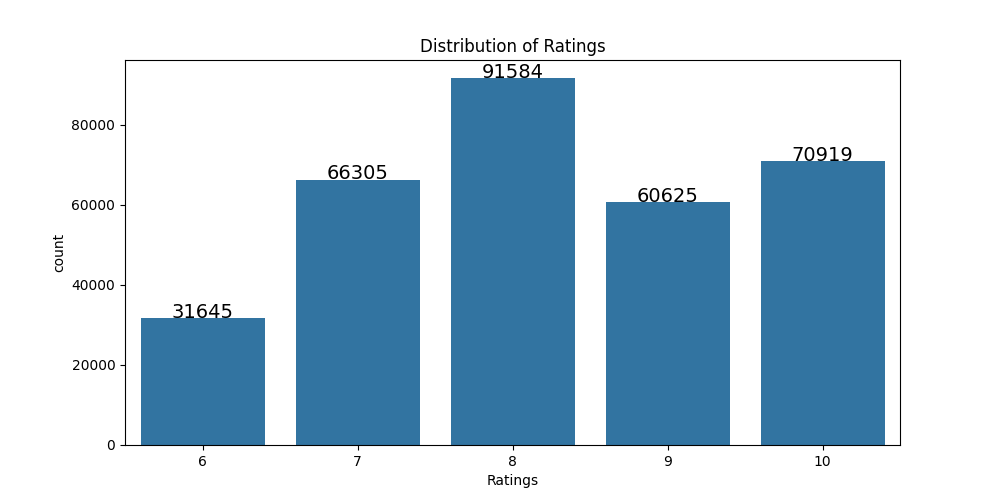
\includegraphics[width=0.9\textwidth]{distribution_of_ratings_after.png} % Remplace 'image.png' par le nom de ton image
    \caption{Distribution des évaluations après le prétraitement}
    \label{fig:mon_image}
\end{figure}


% ********************************************************************************************************************************

\newpage
\pagestyle{fancy}
\section{Extraction de motifs fréquents}
\justifying 

\subsection{Concept et importance dans l'exploration de données}
L'extraction de motifs fréquents (Frequent Pattern Mining) est un processus clé en exploration de données (data mining) qui consiste à identifier des motifs, des séquences ou des ensembles d'éléments qui apparaissent fréquemment dans un ensemble de données. Ces motifs peuvent révéler des tendances cachées dans les données et être utilisés pour diverses applications, comme les systèmes de recommandation, l'analyse de panier d'achat, ou même la détection d'anomalies. L'extraction de motifs fréquents est cruciale car elle permet de comprendre les relations entre les données, d'améliorer la prise de décision, et d'optimiser les processus dans de nombreux domaines, notamment le marketing, la vente, et l'analyse comportementale.

\subsection{Définitions}


\subsubsection{Transactions, items et ensembles d'éléments fréquents (frequent itemsets):}
\begin{itemize}
    \item \textbf{Transactions} : Une transaction dans un contexte d'exploration de données est un enregistrement individuel dans une base de données, souvent représenté par un ensemble d'éléments ou d'objets associés. Par exemple, dans notre système de recommandation de livres, une transaction est la lecture d'un livre par un utilisateur.
    \item \textbf{Items (éléments)} : Un item est un objet individuel ou un élément d'une transaction. Dans le contexte d'une boutique en ligne, un item pourrait être un produit spécifique, comme un livre particulier.
    \item \textbf{Ensembles d'éléments fréquents} : Un ensemble d'éléments fréquent est un groupe d'items qui apparaissent ensemble dans un nombre suffisamment élevé de transactions. L'extraction de ces ensembles est au cœur de l'extraction de motifs fréquents, car ils permettent de découvrir des relations entre les éléments.
    \item \textbf{Ensembles d'éléments candidats} : Un ensemble d'éléments candidats est un groupe d'items qui pourrait potentiellement être fréquent. Ces ensembles sont générés pendant le processus d'exploration de motifs fréquents et nécessitent une validation en calculant leur support pour déterminer s'ils sont effectivement fréquents. Par exemple, si les items \(A\) et \(B\) apparaissent souvent séparément dans les transactions, \( \{A, B\} \) pourrait être un ensemble candidat à évaluer.
\end{itemize}
    
\subsubsection {Support, confiance et lift (mesures clés):}
\begin{itemize}
    \item \textbf{Support} : Le support mesure la fréquence d'apparition d'un ensemble d'éléments dans l'ensemble des transactions. Il est calculé comme le pourcentage de transactions dans lesquelles un ensemble d'éléments donné apparaît. Le support est utilisé pour évaluer la pertinence d'un motif en fonction de sa fréquence dans les données.
    \[
    \text{Support}(A) = \frac{\text{Nombre de transactions contenant } A}{\text{Total des transactions}}
    \]
    \item \textbf{Confiance (Confidence)} : La confiance est une mesure de la probabilité qu'un élément apparaisse dans une transaction, étant donné qu'un autre élément y est présent. Elle est utilisée pour évaluer la force d'une règle d'association. Par exemple, la confiance d'une règle "Si l'utilisateur achète le livre X, alors il achètera aussi le livre Y" est la probabilité d'acheter Y, sachant que X a été acheté.
    \[
    \text{Confiance}(A \rightarrow B) = \frac{\text{Support}(A \cup B)}{\text{Support}(A)}
    \]
    \item \textbf{Lift} : Le lift mesure l'augmentation de la probabilité de trouver deux éléments ensemble par rapport à ce qui serait attendu si les éléments étaient indépendants. Un lift supérieur à 1 indique une forte association entre les éléments, tandis qu'un lift inférieur à 1 suggère qu'ils sont moins susceptibles d'apparaître ensemble que prévu par hasard.
    \[
    \text{Lift}(A \rightarrow B) = \frac{\text{Confiance}(A \rightarrow B)}{\text{Support}(B)}
    \]
\end{itemize}

\subsection{Défis dans l'extraction de motifs}
L'extraction de motifs fréquents présente plusieurs défis importants :
\begin{itemize}
    \item \textbf{Problème de complexité computationnelle} : L'extraction de motifs fréquents peut devenir très coûteuse en termes de temps et de mémoire, en particulier pour de grandes bases de données. La croissance combinatoire du nombre d'ensembles d'éléments possibles rend les calculs inefficaces.
    \item \textbf{Manipulation de données volumineuses et variables} : Les grandes bases de données avec un grand nombre de transactions et d'items rendent difficile l'extraction de motifs fréquents. De plus, les données peuvent être complexes et variées, rendant l'identification de motifs significatifs plus difficile.
    \item \textbf{Sélection des paramètres} : Le choix des seuils de support, de confiance et de lift peut avoir un impact important sur les résultats. Des seuils trop élevés peuvent entraîner la perte de motifs potentiellement intéressants, tandis que des seuils trop faibles peuvent entraîner des motifs trop généraux ou non significatifs.
    \item \textbf{Variabilité des motifs} : Les motifs peuvent varier en fonction des contextes ou des utilisateurs. Il peut être difficile de distinguer les motifs pertinents pour différents segments d'utilisateurs ou contextes d'utilisation.
\end{itemize}

% ********************************************************************************************************************************

\newpage
\pagestyle{fancy}
\section{Techniques et Algorithmes Utilisés}
\justifying 
Pour les recommandations, nous avons utilisé trois techniques populaires basées sur les règles d'association : \textbf{Apriori}, \textbf{Eclat}, et \textbf{FP-Growth}.


%**********************************************************************************************************************
%****************************************HAFSA**********************************************************************

\subsection{Apriori}




%************************************************************************************************************************************
%*********************************************FIRDAWS******************************************************************************
%***********************************************************************************************************************************
\subsection{Eclat}

\subsection{FP-Growth}

\subsubsection{Algorithme FP-Growth : Une Version Améliorée de l'Apriori:}

L'algorithme \textbf{FP-Growth} (Frequent Pattern Growth) est une version améliorée de l'algorithme \textbf{Apriori}, spécialement conçu pour surmonter certaines des limitations d'Apriori, en particulier son inefficacité en termes de coûts computationnels et d'utilisation de mémoire. FP-Growth est plus efficace car il évite la génération de candidats d'ensembles d'éléments fréquents (itemsets) comme le fait l'algorithme Apriori. Au lieu de cela, FP-Growth utilise une structure de données compacte appelée \textbf{l'arbre FP} (Frequent Pattern Tree) et extrait directement les ensembles d'éléments fréquents à partir de cet arbre. Voici une explication détaillée de l'algorithme FP-Growth avec un exemple à partir d'un jeu de données aléatoire.

\subsubsection{Différences Clés entre Apriori et FP-Growth:}
\begin{itemize}
    \item \textbf{Génération de Candidats} : 
    \begin{itemize}
        \item \textbf{Apriori} génère des candidats d'ensembles d'éléments fréquents à chaque itération et les taille ensuite en fonction du seuil de support minimum.
        \item \textbf{FP-Growth} évite la génération de candidats et utilise une structure d'arbre efficace pour découvrir les ensembles fréquents d'éléments.
    \end{itemize}
    
    \item \textbf{Efficacité} :
    \begin{itemize}
        \item \textbf{Apriori} nécessite plusieurs passages sur l'ensemble des données, à chaque fois en générant des ensembles candidats de plus en plus grands.
        \item \textbf{FP-Growth} ne nécessite que deux passages sur le jeu de données : un pour construire l'arbre FP et un autre pour exploiter cet arbre.
    \end{itemize}
\end{itemize}

\subsubsection{Explication de l'Algorithme FP-Growth}

\textbf{Étape 1 : Construction de l'Arbre FP}

L'arbre FP est une représentation compressée du jeu de données. Il stocke les ensembles d'éléments fréquents dans une structure en arbre, où les chemins de l'arbre représentent les combinaisons d'ensembles d'éléments.

\begin{itemize}
    \item \textbf{Nœud Racine} : Représente un ensemble vide.
    \item \textbf{Nœuds Enfants} : Représentent les éléments du jeu de données.
    \item \textbf{Arêtes} : Représentent les fréquences des éléments.
\end{itemize}

\textbf{Étape 2 : Extraction des Ensembles Fréquents à Partir de l'Arbre FP}

Une fois l'arbre FP construit, l'algorithme utilise cet arbre pour trouver les ensembles d'éléments fréquents. À partir du bas de l'arbre (les éléments ayant les plus faibles supports), il trace des chemins jusqu'à la racine pour découvrir les ensembles fréquents d'éléments.

\subsubsection{Exemple Pratique}

Prenons un \textbf{jeu de données aléatoire} :

\renewcommand{\arraystretch}{1.5}

\begin{longtable}{|l|l|}
\hline
\textbf{ID Transaction} & \textbf{Livres} \\
\hline
\endfirsthead
\hline
T1 & \{A, B, D, E\} \\
T2 & \{B, D, E\} \\
T3 & \{A, B, D\} \\
T4 & \{B, E\} \\
T5 & \{A, D, E, F\} \\
\hline
\end{longtable}

\textbf{Étape 1 : Prétraitement du Jeu de Données}

\begin{itemize}
    \item \textbf{Calcul des fréquences des éléments} (compte de support pour chaque élément) :
    
    \begin{longtable}{|l|c|c|c|c|c|}
    \hline
    \textbf{ID Transaction} & \textbf{A} & \textbf{B} & \textbf{D} & \textbf{E} & \textbf{F} \\
    \hline
    \endfirsthead
    \hline
    T1 & 1 & \ 1 & \ 1 & \ 1 & \ 0 \\
    \hline
    T2 & 0 & \ 1 & \ 1 & \ 1 & \ 0 \\
    \hline
    T3 & 1 & \ 1 & \ 1 & \ 0 & \ 0 \\
    \hline
    T4 & 0 & \ 1 & \ 0 & \ 1 & \ 0 \\
    \hline
    T5 & 1 & \ 0 & \ 1 & \ 1 & \ 1 \\
    \hline
    \end{longtable}
    
    \[
    \text{Support(livre)} = \sum_{i=1}^{n} \text{Présence du livre dans la transaction } T_i
    \]

    \textbf{avec :}
    \begin{itemize}
        \item \(n\) représente le nombre total de transactions dans le jeu de données.
        \item La présence d'un livre dans une transaction est indiquée par 1, et l'absence par 0.
    \end{itemize}

    \textbf{Exemple avec le livre \(A\) :}
    \[
    \text{Support(A)} = \text{Présence dans } T1 + \text{Présence dans } T2 + \text{...} + \text{Présence dans } T5
    \]
    \[
    \text{Support(A)} = 1 + 0 + 1 + 0 + 1 = 3
    \]

    De la même manière, nous pouvons calculer les supports pour les autres livres :
    \begin{align*}
    \text{Support(B)} & = 1 + 1 + 1 + 1 + 0 = 4 \\
    \text{Support(D)} & = 1 + 1 + 1 + 0 + 1 = 4 \\
    \text{Support(E)} & = 1 + 1 + 0 + 1 + 1 = 4 \\
    \text{Support(F)} & = 0 + 0 + 0 + 0 + 1 = 1
    \end{align*}

    \item \textbf{Application du seuil de support minimum} (disons que le support minimum = 3). Les éléments dont le support est inférieur à 3 sont éliminés, ce qui donne :
    \begin{itemize}
        \item A, B, D, E.
    \end{itemize}
    
    \item \textbf{Tri des éléments} : On trie les éléments selon leur fréquence dans les transactions. Le tri donne l'ordre suivant (du plus fréquent au moins fréquent) :
    \begin{itemize}
        \item B (4), D (4), E (4), A (3).
    \end{itemize}
\end{itemize}

\textbf{Étape 2 : Construction de l'Arbre FP}

L'arbre FP est construit en ajoutant les transactions de manière compressée. Chaque transaction est ajoutée de manière à ce que les éléments soient triés dans l'ordre des éléments les plus fréquents. Les transactions peuvent partager des préfixes communs dans l'arbre, ce qui permet une compression des données.

\textbf{Transactions après suppression des éléments peu fréquents (F) et triées par fréquence des éléments :}

\begin{longtable}{|c|c|}
\hline
\textbf{ID Transaction} & \textbf{Livres} \\
\hline
T1 & \{B, D, E, A\} \\
T2 & \{B, D, E\} \\
T3 & \{B, D, A\} \\
T4 & \{B, E\} \\
T5 & \{D, E, A\} \\
\hline
\end{longtable}

\textbf{Construction de l'arbre FP} :

\begin{center}
\begin{tikzpicture}[
  every node/.style={fill=blue!20,rounded corners},
  level 1/.style={sibling distance=5cm},
  level 2/.style={sibling distance=4cm},
  level 3/.style={sibling distance=3cm}
  level 4/.style={sibling distance=2cm}
  ]
  \node {}
    child {node {B(4)}
      child {node {D(3)}
        child {node {E(2)}
          child {node {A(1)}}
        }    
        child {node {A(1)}}
      }
      child {node {E(1)}}
    }
    child {node {D(1)}
      child {node {E(1)}
        child {node {A(1)}}
      }
    };
\end{tikzpicture}
\end{center}

\textbf{Étape 3 : Extraction des Ensembles Fréquents à partir de l'Arbre FP}

Une fois l'arbre FP construit, on peut en extraire les ensembles fréquents d'éléments en suivant les chemins de l'arbre. Chaque chemin correspond à un ensemble d'éléments fréquents, et les combinaisons possibles sont extraites en remontant l'arbre. En appliquant cet algorithme à notre ensemble de données, nous serons capables d'identifier des règles d'association réelles basées sur les habitudes de lecture des utilisateurs. Ces règles associent des livres qui sont fréquemment lus ensemble, ce qui peut être utilisé pour générer des recommandations. Par exemple, si une règle fréquente de type {Livre A, Livre B} $\rightarrow$ {Livre C} est extraite, cela signifie qu'un utilisateur ayant lu les livres A et B est susceptible de lire également le livre C.

\subsubsection{Pseudo-Code de l'Algorithme FP-Growth}

Voici un pseudo-code simple de l'algorithme FP-Growth :

\begin{algorithm}[H]
\SetAlgoLined
\KwData{Un ensemble de transactions avec des éléments}
\KwResult{Ensembles d'éléments fréquents}
\KwIn{$min\_support$: Seuil minimum de support}
\KwOut{Ensembles d'éléments fréquents ayant un support supérieur ou égal à $min\_support$}
  
\For{élément \textbf{$i$} dans l'ensemble de données}{
    \textbf{Compter} la fréquence de $i$
}
\For{ensemble d'éléments \textbf{$I$}}{
    \textbf{Construire l'arbre FP} en insérant les ensembles d'éléments dans la structure de l'arbre selon la fréquence et l'ordre des éléments
}
\For{modèle fréquent dans l'arbre FP}{
    \textbf{Générer la base de motifs conditionnels} en extrayant les sous-ensembles des modèles fréquents \\
    \textbf{Générer l'arbre FP conditionnel} en appliquant de manière récursive l'algorithme FP-Growth sur la base de motifs conditionnels
}
\caption{Algorithme FP-Growth}
\end{algorithm}



    





%**********************************************************************************************************************************
\newpage
\section{Étude Comparative et Sélection du Meilleur Modèle}
\justifying

Après avoir appliqué les algorithmes Apriori, Eclat, et FP-Growth, nous avons comparé leurs performances afin de sélectionner le modèle le plus adapté pour notre système de recommandation. Cette comparaison s'est basée sur plusieurs critères essentiels :

   \textbf{Temps d'exécution} : Chaque algorithme a été évalué en termes de temps nécessaire pour traiter le dataset final et générer les règles d'association.

    \textbf{Nombre de règles extraites} : Nous avons analysé la quantité de règles générées par chaque algorithme, en prenant en compte leur pertinence et leur diversité.

    \textbf{Simplicité des règles} : Un autre critère a été la lisibilité et la simplicité des règles d'association pour leur interprétation par les utilisateurs.

   \textbf{Support et confiance minimaux} : Les valeurs de support et de confiance minimaux influencent directement la qualité des recommandations. Ces paramètres ont été ajustés pour chaque algorithme afin de garantir des résultats optimaux.

\subsection{Résultats Comparatifs}

    \textbf{Apriori} : Cet algorithme a généré des règles d'association pertinentes, mais il était le plus lent en termes de temps d'exécution, surtout avec des datasets de grande taille.

    \textbf{Eclat} : Bien que plus rapide qu’Apriori, Eclat a parfois produit des règles légèrement redondantes, nécessitant un filtrage supplémentaire.

    \textbf{FP-Growth} : Cet algorithme s’est distingué par son efficacité, générant rapidement des règles pertinentes avec une utilisation optimale des ressources.

\subsection{Meilleur Modèle Sélectionné}

Sur la base des résultats obtenus, FP-Growth a été identifié comme le meilleur modèle. Les critères principaux pour ce choix ont été :
\begin{itemize}[label=\textbullet]
    \item Son temps d'exécution rapide sur des datasets volumineux.
    \item La pertinence des règles générées.
    \item Sa capacité à s’adapter aux variations des paramètres comme le support et la confiance minimaux.
\end{itemize}











\end{document}









